\appendix
\addcontentsline{toc}{section}{Appendices}
\section*{\centering{Appendices}}
 \pagenumbering{roman}
 \section{Stewart Platform and Wind Tunnel Configurations}
 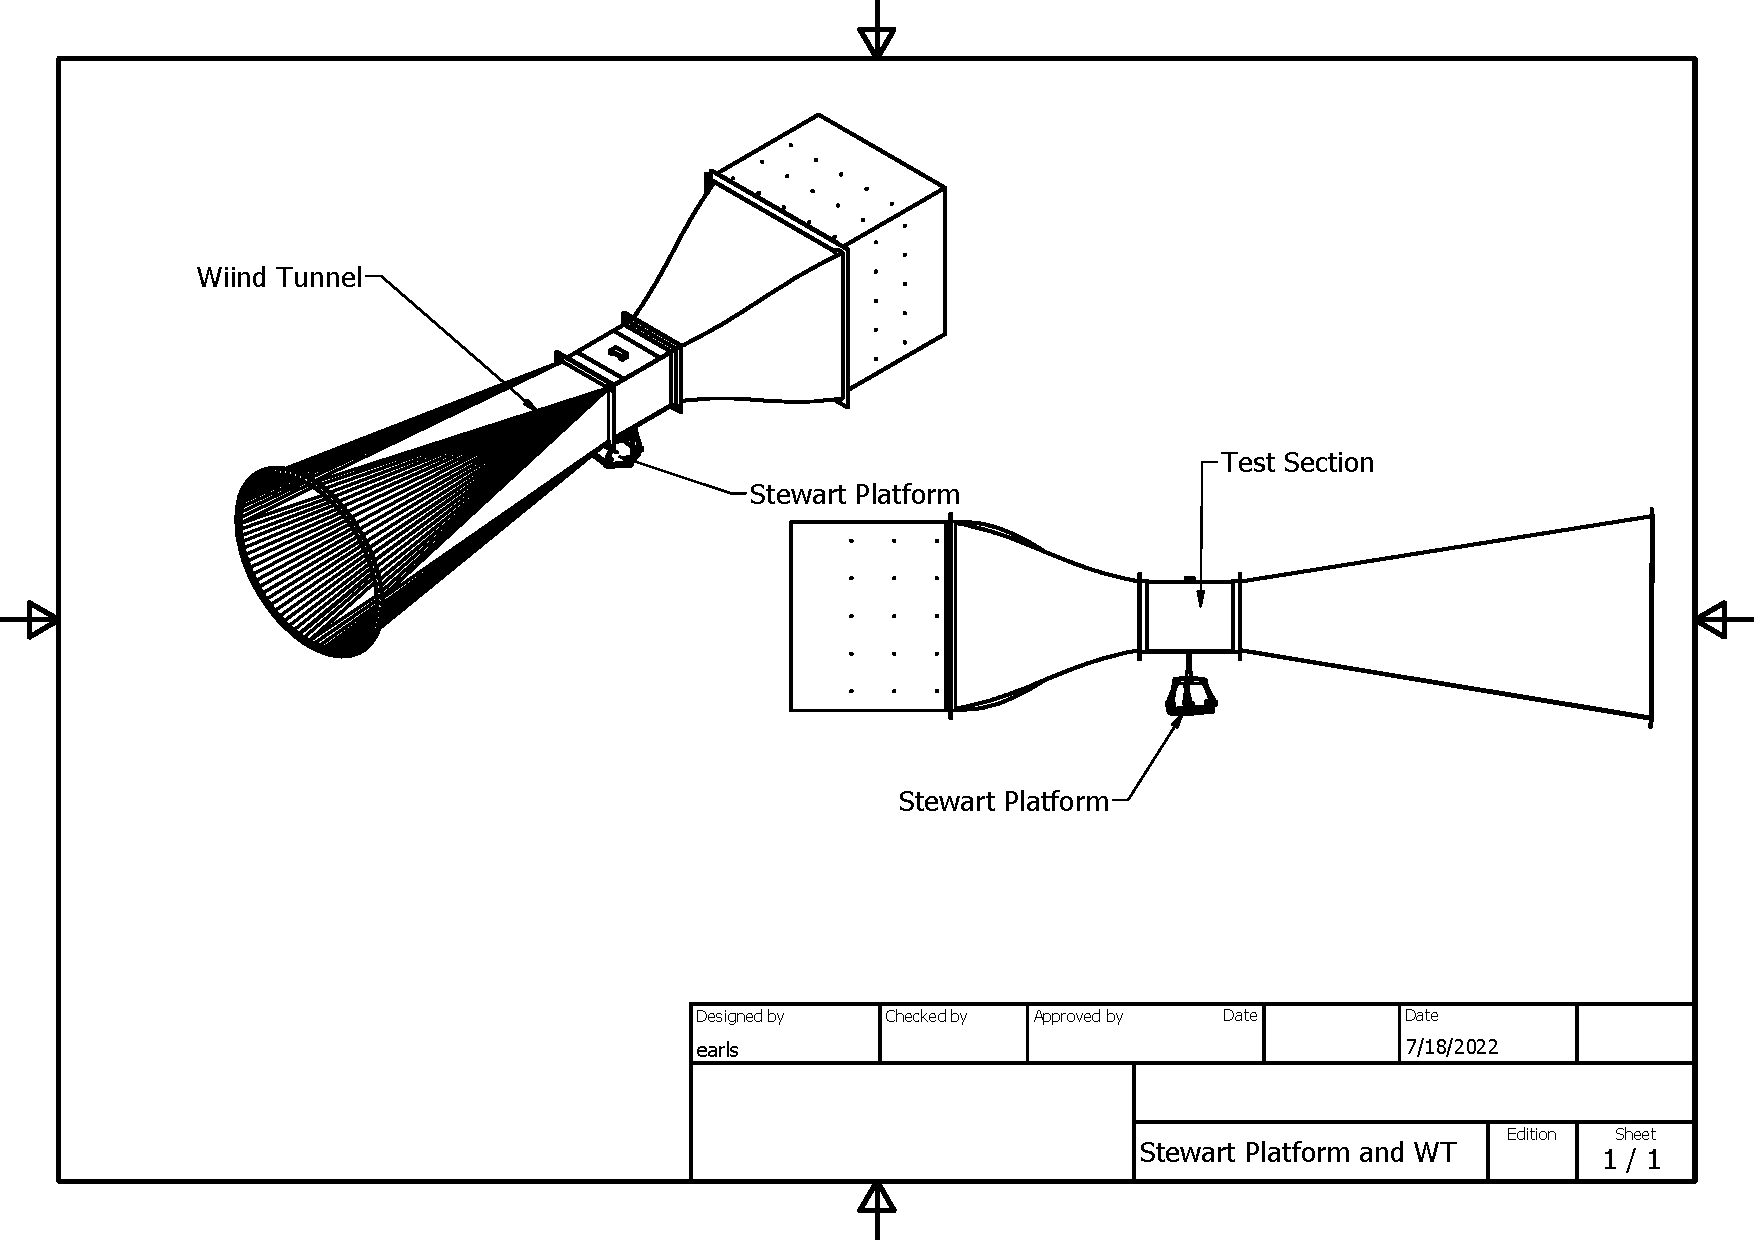
\includepdf[pages=-]{Wind Tunnel Assembly + Stewart}
 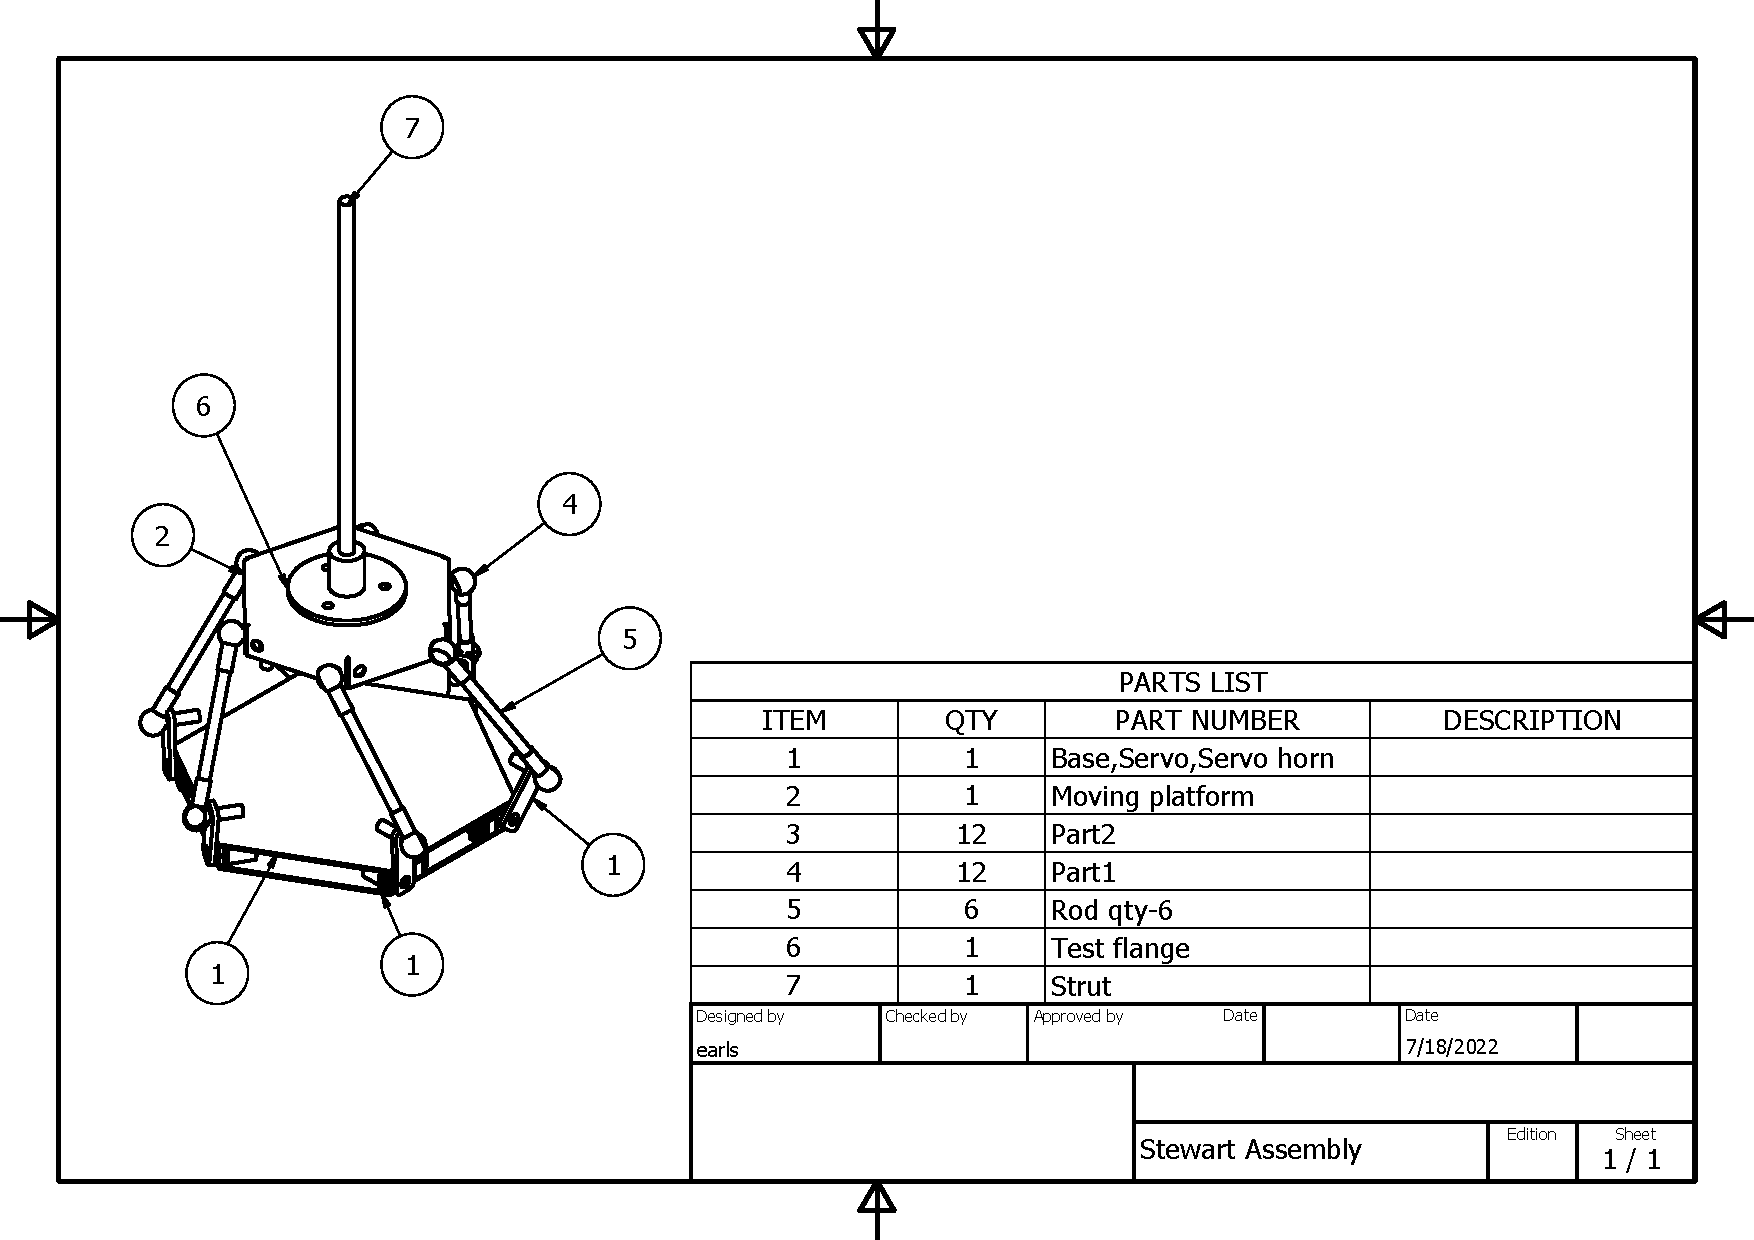
\includepdf[pages=-]{Assemby 3 2}
 \section{Budget and Timeplan}
 \subsection{Provisional Budget}
 \begin{center}
 \begin{table}[!h]
 \centering
 \caption{Proposed budget}
 \paragraph{ }
 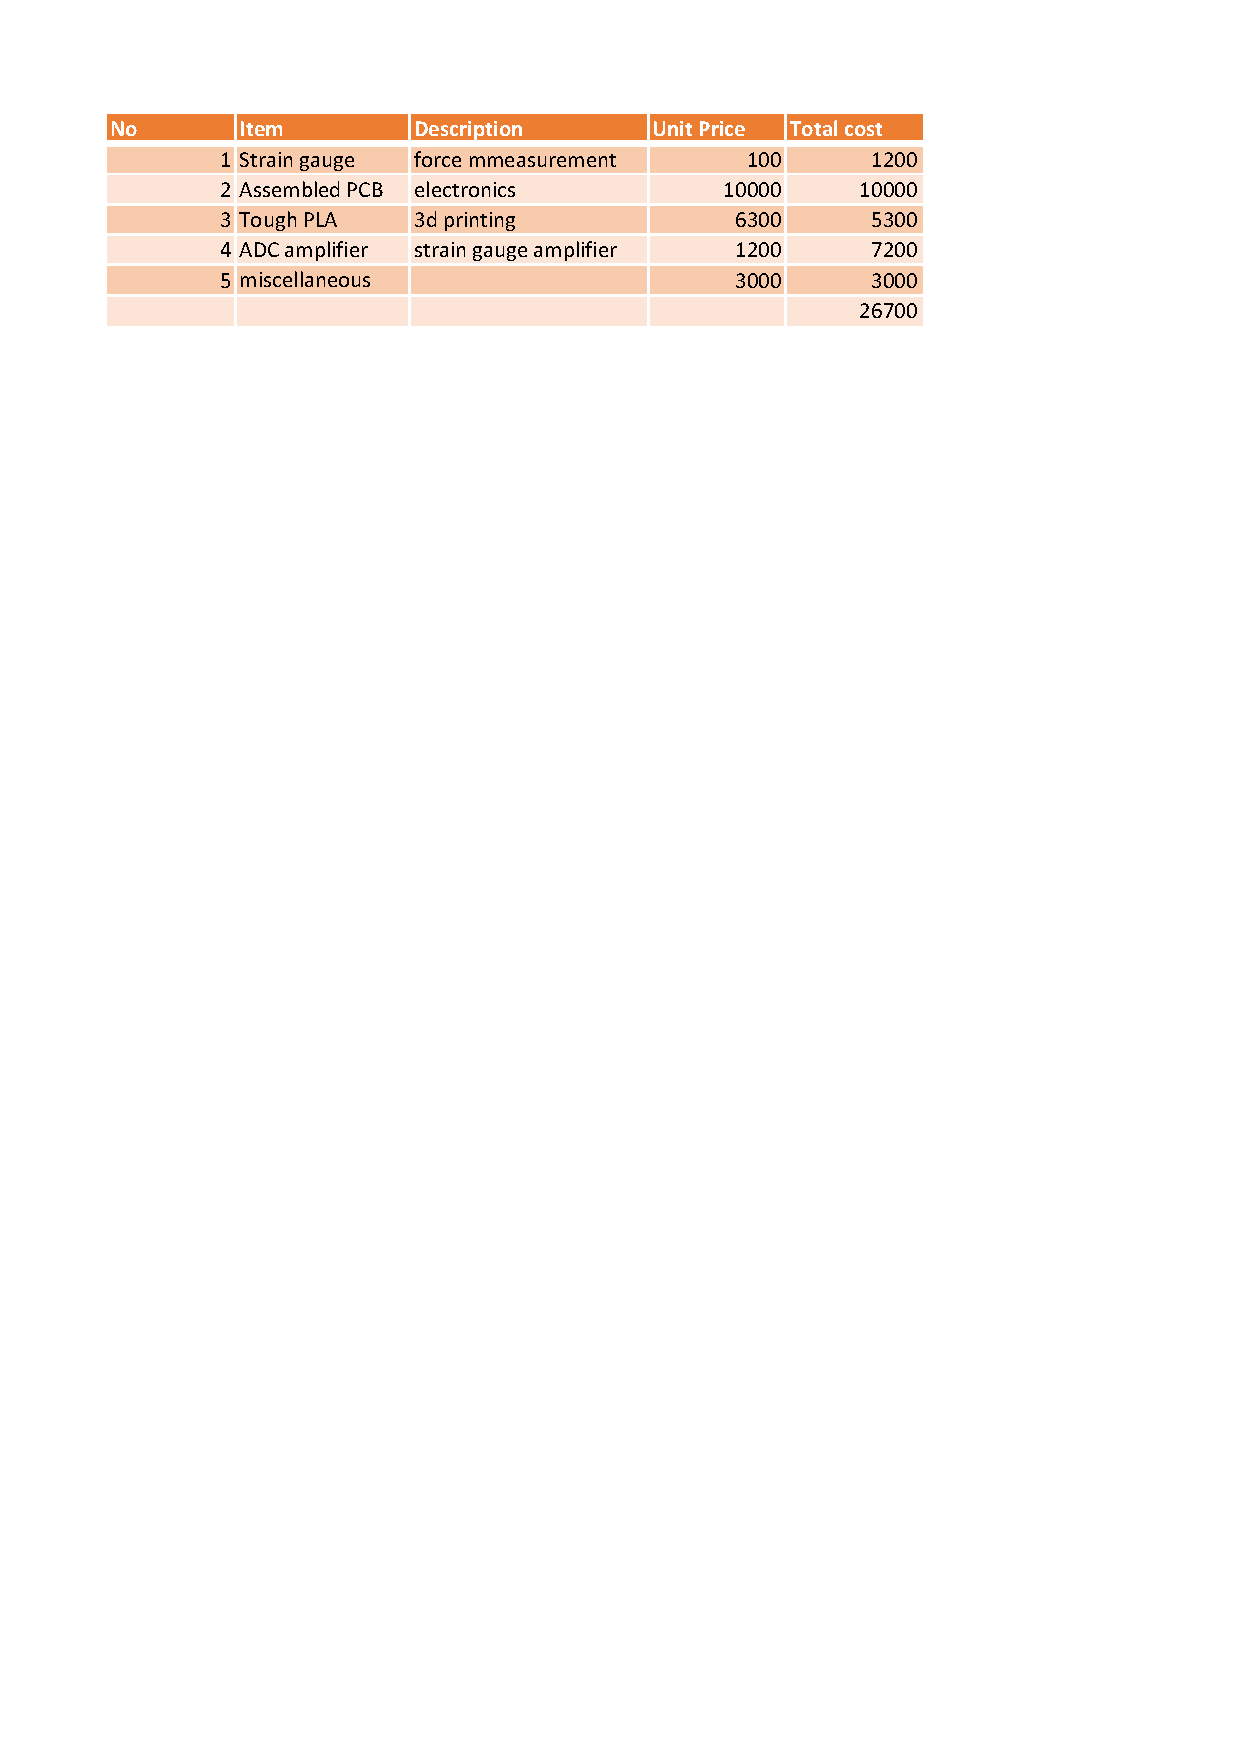
\includegraphics{Figures/budget}
 \end{table}
 \end{center}
 \clearpage
 \subsection{Work Plan}
 \begin{center}
 \begin{table}[!h]
 \centering
 \caption[Time plan]{Time plan for first and second semester}
 \paragraph{ }
 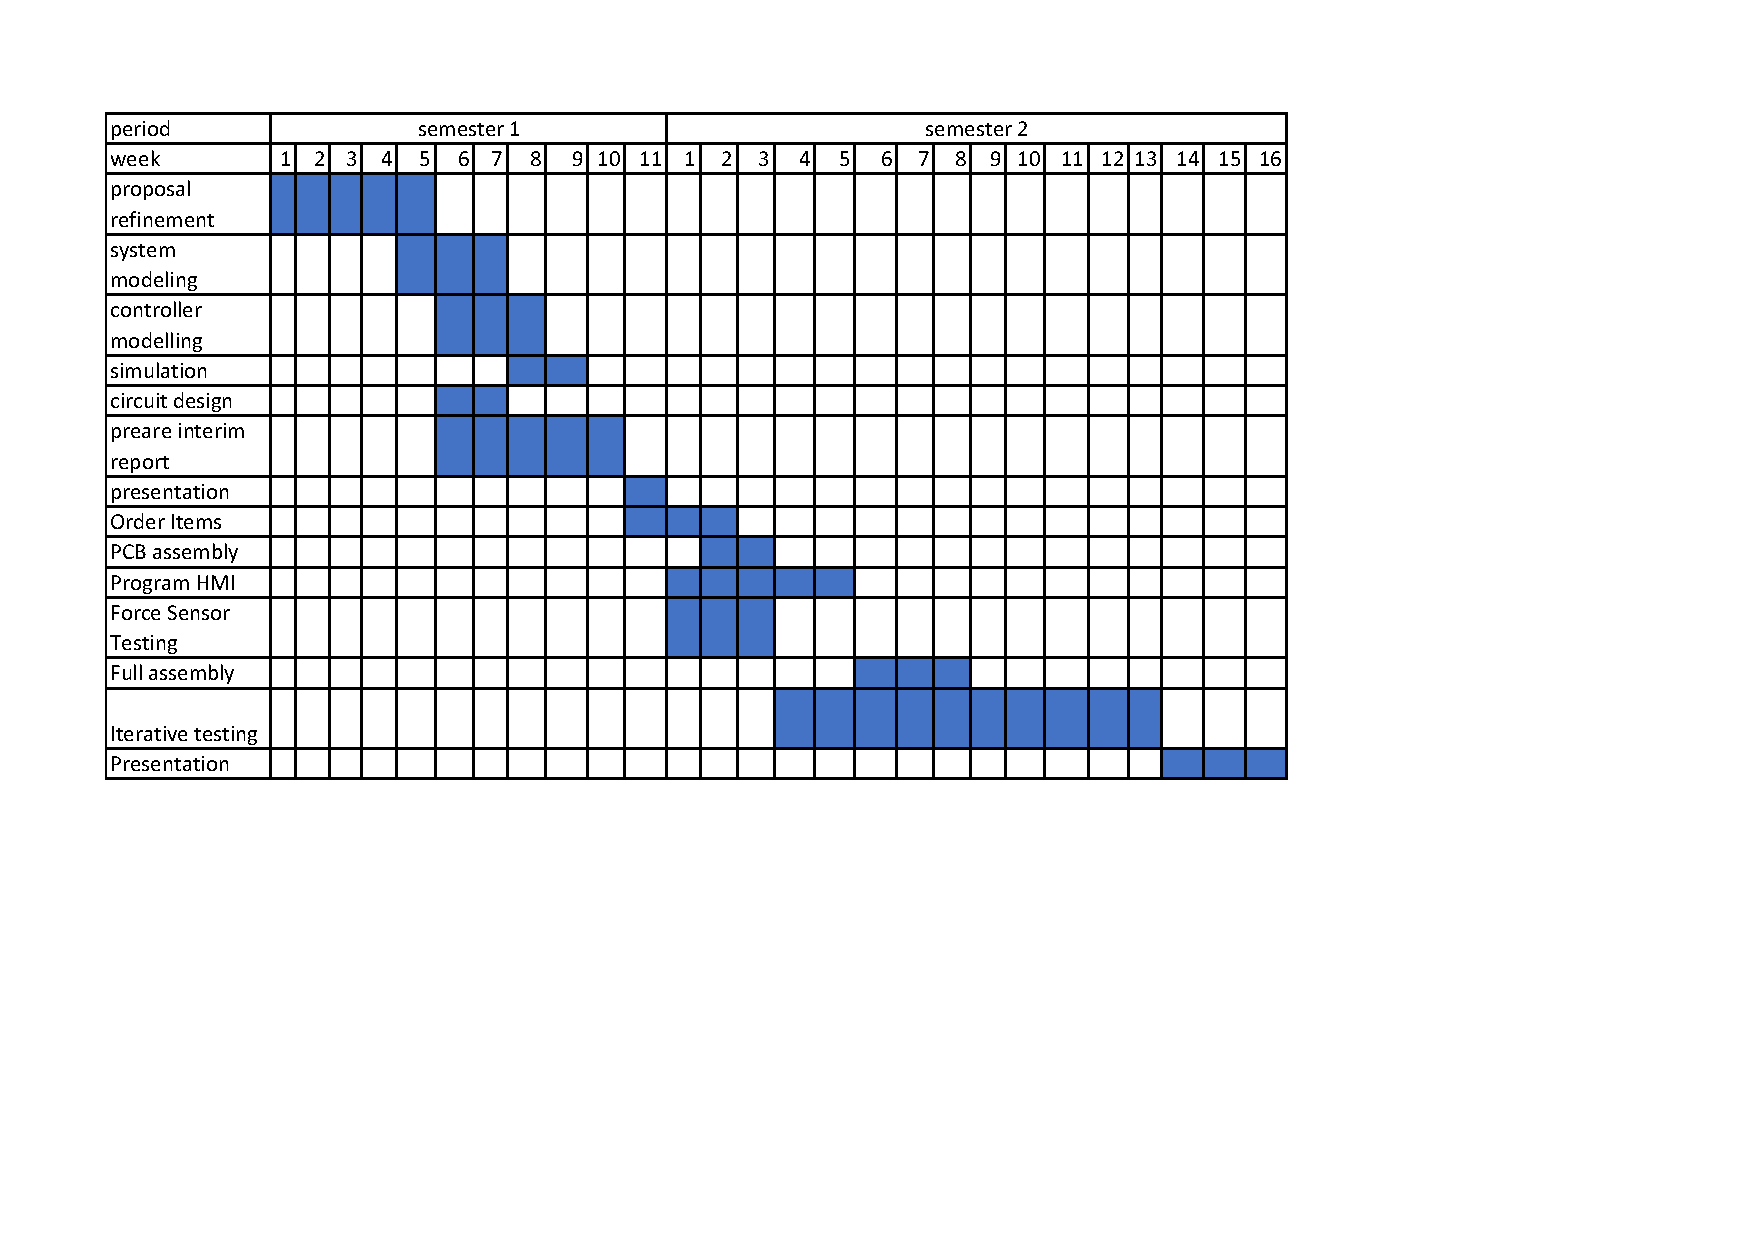
\includegraphics[width=0.95\linewidth]{Figures/workplan}
 \end{table}
 \end{center}
 \clearpage
 
\section{Force transformation matrix} 
In such a case the forces experienced at the top of the platform are distributed between the 6 legs and as result, a force transformation matrix is required to resolve the forces applied on each axis as measured by each load cell on each leg. 

If the platform is acted upon by an external wrench {$\vec{F}_e, \vec{M}_e$}, for static equilibrium of the body, the external wrench is statically balanced by the six leg forces of the Stewart platform. Representing the unit vector $\hat{I}_i$ along the i-th leg with respect to B, the leg force is given  by $\hat{I}_if_i$. Considering the force equilibrium of the platform along  three mutually perpendicular directions in B(XYZ), the following force equations can be obtained as in \cite{dwarakanath_design_2001}:

\begin{ceqn}
	\begin{align}
	(F_e)_x = f_1I_{1x} + f_2I_{2x} + f_3I_{3x} + f_4I_{4x} + f_5I_{5x} + f_6I_{6x}
\end{align}
\end{ceqn}
\begin{ceqn}
	\begin{align}
	(F_e)_y = f_1I_{1y} + f_2I_{2y} + f_3I_{3y} + f_4I_{4y} + f_5I_{5y} + f_6I_{6y}
\end{align}
\end{ceqn}
\begin{ceqn}
	\begin{align}
	(F_e)_z = f_1I_{1z} + f_2I_{2z} + f_3I_{3z} + f_4I_{4z} + f_5I_{5z} + f_6I_{6z}
\end{align}
\end{ceqn}
where $(F_e)_x$, $(F_e)_y$ and $(F_e)_z$ are the external forces on the platform along three mutually perpendicular directions x, y and z of the frame B, respectively.

The moment due to the forces $\hat{I}_if_i$ about the origin of B is $(\vec{b}_i x \hat{I}_i)f_i$. Considering the moment equilibrium about x, y and z axes of B, the following moment equations can be obtained as in \cite{dwarakanath_design_2001}:

\begin{ceqn}
	\begin{align}
	(M_e)_x = f_1(\vec{b}_1 x \hat{I}_1)_x + f_2(\vec{b}_2 x \hat{I}_2)_x + f_3(\vec{b}_3 x \hat{I}_3)_x + f_4(\vec{b}_4 x \hat{I}_4)_x + f_5(\vec{b}_5 x \hat{I}_5)_x + f_6(\vec{b}_6 x \hat{I}_6)_x
\end{align}
\end{ceqn}
\begin{ceqn}
	\begin{align}
	(M_e)_y = f_1(\vec{b}_1 x \hat{I}_1)_y + f_2(\vec{b}_2 x \hat{I}_2)_y + f_3(\vec{b}_3 x \hat{I}_3)_y + f_4(\vec{b}_4 x \hat{I}_4)_y + f_5(\vec{b}_5 x \hat{I}_5)_y + f_6(\vec{b}_6 x \hat{I}_6)_y
	\end{align}
\end{ceqn}
\begin{ceqn}
	\begin{align}
	(M_e)_z = f_1(\vec{b}_1 x \hat{I}_1)_z + f_2(\vec{b}_2 x \hat{I}_2)_z + f_3(\vec{b}_3 x \hat{I}_3)_z + f_4(\vec{b}_4 x \hat{I}_4)_z + f_5(\vec{b}_5 x \hat{I}_5)_z + f_6(\vec{b}_6 x \hat{I}_6)_z
	\end{align}
\end{ceqn}

where $(M_e)_x$, $(M_e)_y$ and $(M_e)_z$ are the external moments on the platform  about the three coordinate axes of B. Combining the equations the relationship between the external wrench and the forces experienced by the legs can be expressed as follows:
\begin{ceqn}
\begin{align}
	\begin{Bmatrix}
		\vec{F}_e \\
		\vec{M}_e \\
	\end{Bmatrix} = [H]\{F\}
\end{align}
\end{ceqn}
\clearpage
\section{HMI code}
 \subsection{Program}
 \begin{verbatim}
 package main
 
 import (
 	"fmt"
 	"math"
 
 	g "github.com/AllenDang/giu"
 )
 
 var (
 	yaw         int32
 	pitch       int32
 	roll        int32
 	transx      int32
 	transy      int32
 	transz      int32
 	tabwidth    float32 = 350
 	tabheight   float32 = 150
 	leg1        []float64
 	leg2        []float64
 	leg3        []float64
 	leg4        []float64
 	leg5        []float64
 	leg6        []float64
 	lineTicks   []g.PlotTicker
 	airVelocity []float64
 )
 
 func loop() {
 	g.SingleWindowWithMenuBar().Layout(
 		g.SplitLayout(g.DirectionVertical, tabheight,
 			g.SplitLayout(g.DirectionHorizontal, tabwidth,
 				g.Layout{
 					g.Label("Rotation Angles"),
 					g.Row(
 						g.VSliderInt(&yaw, -5, 5).Label("Yaw").Size(40, 110).OnChange(func() { fmt.Println(yaw) }),
 						g.VSliderInt(&pitch, -5, 5).Label("Pitch").Size(40, 110),
 						g.VSliderInt(&roll, -5, 5).Label("Roll").Size(40, 110),
 					),
 				},
 				g.SplitLayout(g.DirectionHorizontal, tabwidth,
 					g.Layout{
 						g.Label("Translations (mm)"),
 						g.Row(
 							g.VSliderInt(&transx, -5, 5).Label("X").Size(40, 110).OnChange(func() { fmt.Println(yaw) }),
 							g.VSliderInt(&transy, -5, 5).Label("Y").Size(40, 110),
 							g.VSliderInt(&transz, -5, 5).Label("Z").Size(40, 110),
 						),
 					},
 					g.Layout{
 						g.Row(
 							g.Button("Home Platform").Size(120, 100),
 							g.Button("Write Position").Size(120, 100),
 							g.Button("Record Data").Size(120, 100),
 						),
 					},
 				),
 			),
 			g.Layout{
 				g.Plot("Strain Data").AxisLimits(0, 100, -1.2, 1.2, g.ConditionOnce).XTicks(lineTicks, false).Plots(
 					g.PlotLine("Leg 1", leg1),
 					g.PlotLine("Leg 2", leg2),
 					g.PlotLine("Leg 3", leg3),
 					g.PlotLine("Leg 4", leg4),
 					g.PlotLine("Leg 5", leg5),
 					g.PlotLine("Leg 6", leg6),
 				),
 				g.Plot("Air velocity").AxisLimits(0, 100, -2, 2, g.ConditionOnce).XTicks(lineTicks, false).Plots(
 					g.PlotScatter("velocity(m/s)", airVelocity),
 				),
 			},
 		),
 	)
 }
 
 func main() {
 	for x := 0.0; x < 10; x += 0.1 {
 		leg1 = append(leg1, math.Sin(x))
 		leg2 = append(leg2, math.Cos(x))
 		leg3 = append(leg3, math.Sin(x)+0.1)
 		leg4 = append(leg4, math.Cos(x)+0.1)
 		leg5 = append(leg5, math.Sin(x)+0.3)
 		leg6 = append(leg6, math.Cos(x)+0.3)
 	}
 	for x := 0.0; x < 10; x += 0.1 {
 		airVelocity = append(airVelocity, 1.5)
 	}
 	w := g.NewMasterWindow("Overview", 1300, 700, 0)
 	w.Run(loop)
 }
 
 \end{verbatim}
 
 \section{PCB schematics}
 \subsection{schematics}
 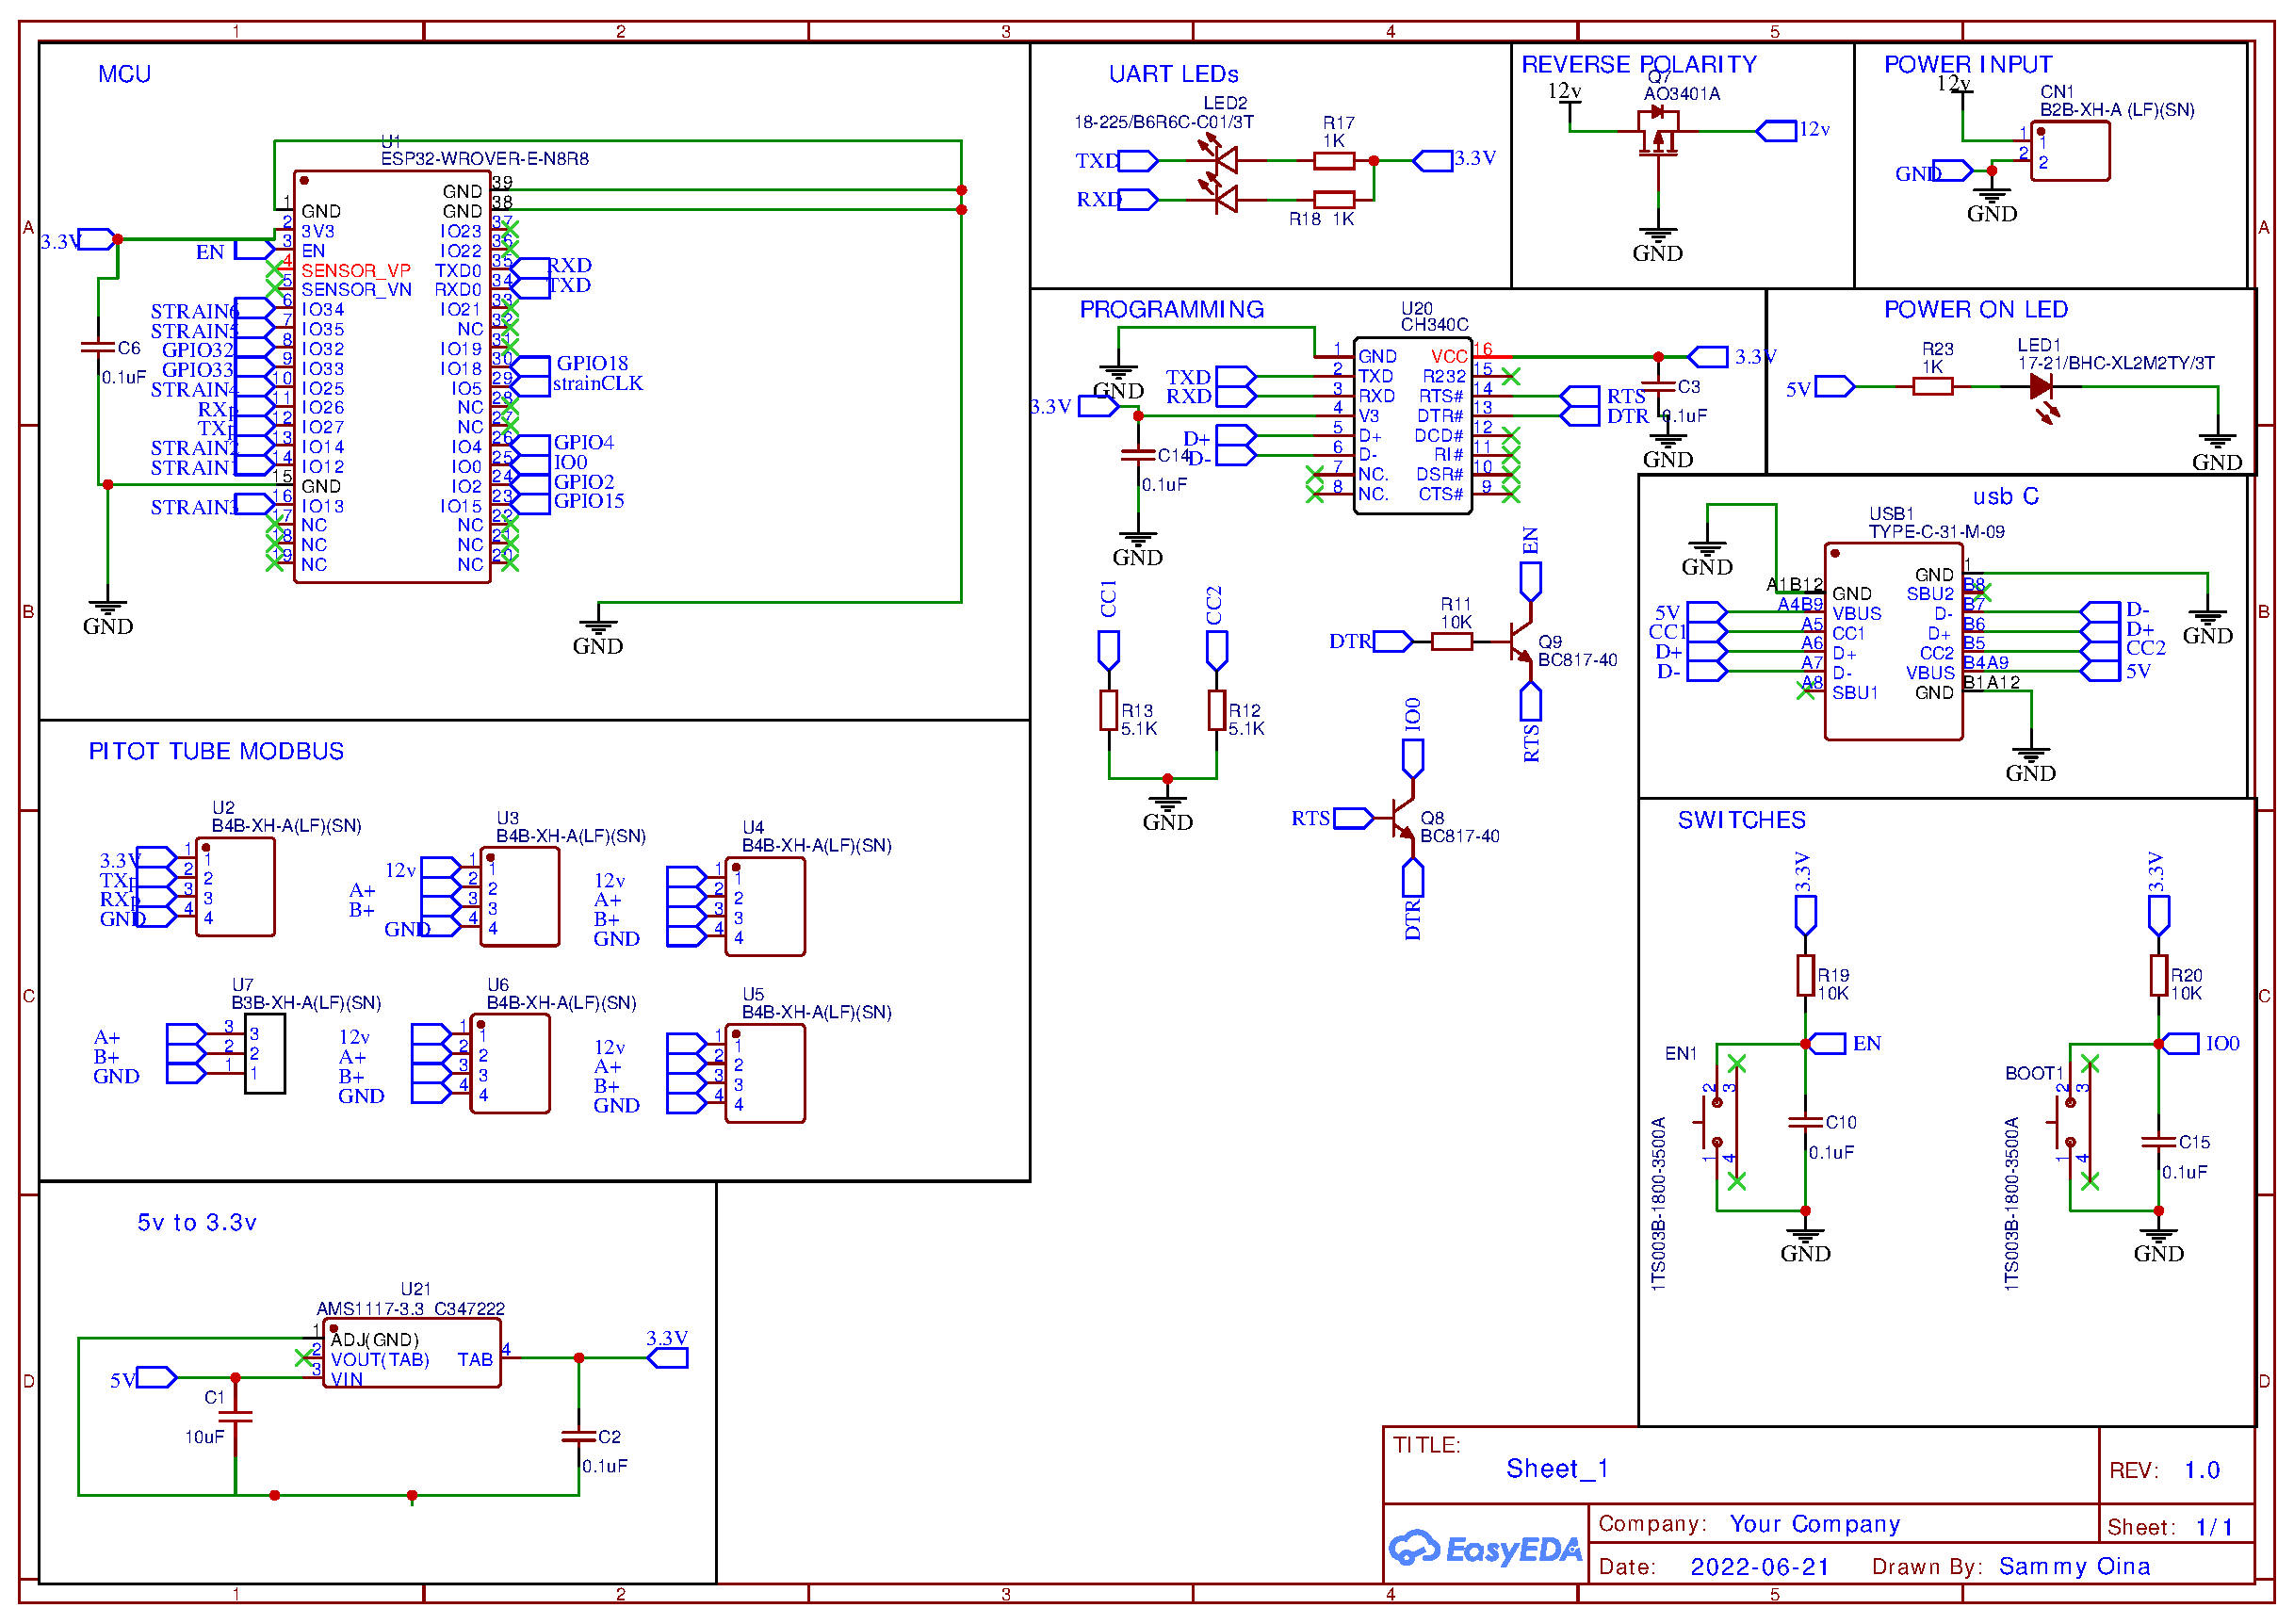
\includepdf[pages=-]{Figures/schm}